\documentclass[12pt]{article}
\usepackage[letterpaper, total={6in, 8in}]{geometry}
\setlength{\oddsidemargin}{0in}
\setlength{\evensidemargin}{0in}
\setlength{\textwidth}{6.5in}
\setlength{\parindent}{0in}
\setlength{\parskip}{\baselineskip}

\usepackage{amsmath,amsfonts,amssymb}
\usepackage{subfigure}
\usepackage{sectsty}
\usepackage{multirow}
\usepackage{makecell}
\usepackage{float}
\usepackage[utf8x]{inputenc}
\usepackage[pdftex]{graphicx}
\usepackage[toc,page]{appendix}
\usepackage{enumitem}
\usepackage{indentfirst}
\usepackage{scrextend}
\usepackage{caption}
\usepackage{hyperref}

\usepackage{listings}
\usepackage{color} %red, green, blue, yellow, cyan, magenta, black, white
\definecolor{mygreen}{RGB}{28,172,0} % color values Red, Green, Blue
\definecolor{mylilas}{RGB}{170,55,241}

\DeclareFixedFont{\ttb}{T1}{txtt}{bx}{n}{10} % for bold
\DeclareFixedFont{\ttm}{T1}{txtt}{m}{n}{10}  % for normal

\usepackage{color}
\definecolor{deepblue}{rgb}{0,0,0.5}
\definecolor{deepred}{rgb}{0.6,0,0}
\definecolor{deepgreen}{rgb}{0,0.5,0}

\usepackage{listings}
\lstset{language=Matlab,%
	%basicstyle=\color{red},
	breaklines=true,%
	morekeywords={matlab2tikz},
	keywordstyle=\color{blue},%
	morekeywords=[2]{1}, keywordstyle=[2]{\color{black}},
	identifierstyle=\color{black},%
	stringstyle=\color{mylilas},
	commentstyle=\color{mygreen},%
	showstringspaces=false,%without this there will be a symbol in the places where there is a space
	numbers=left,%
	numberstyle={\tiny \color{black}},% size of the numbers
	numbersep=9pt, % this defines how far the numbers are from the text
	emph=[1]{for,end,break},emphstyle=[1]\color{red}, %some words to emphasise
	%emph=[2]{word1,word2}, emphstyle=[2]{style},    
}


% Python style for highlighting
\newcommand\pythonstyle{\lstset{
		language=Python,
		basicstyle=\ttm,
		otherkeywords={self},             % Add keywords here
		keywordstyle=\ttb\color{deepblue},
		emph={MyClass,__init__},          % Custom highlighting
		emphstyle=\ttb\color{deepred},    % Custom highlighting style
		stringstyle=\color{deepgreen},
		frame=tb,                         % Any extra options here
		showstringspaces=false            % 
}}


% Python environment
\lstnewenvironment{python}[1][]
{
	\pythonstyle
	\lstset{#1}
}
{}

% Python for external files
\newcommand\pythonexternal[2][]{{
		\pythonstyle
		\lstinputlisting[#1]{#2}}}

% Python for inline
\newcommand\pythoninline[1]{{\pythonstyle\lstinline!#1!}}

\begin{document}
\hfill Sam Feig $|$ Vladimir Zhdanov \\
\textbf{H3}\hfill CSCI 4831/5722 \\
\rule{\textwidth}{.75pt}

\begin{enumerate}
	\item 
	\begin{enumerate}
		\item This proof will be shown for the $3*3$ kernel size but is the same for any $k > 1$. Consider the following separable 2D filter kernel $g$ of size $2k + 1$ with $k = 1$.
		\begin{align*}
		g_1 &= \begin{bmatrix} w_4 & w_5 & w_6 \end{bmatrix} \\
		g_2 &= \begin{bmatrix} w_1 \\ w_2 \\ w_3 \end{bmatrix} \\
		g &= g_2g_1 \\  
		&= \begin{bmatrix}
		w_1w_4 & w_1w_5 & w_1w_6 \\
		w_2w_4 & w_2w_5 & w_2w_6 \\
		w_3w_4 & w_3w_5 & w_3w_6 
		\end{bmatrix}
		\end{align*}
		Then, consider the following value for our "image" $f$, where the pixel of interest for this proof is $x$.
		\begin{align*}
		f &= \begin{bmatrix}
		a_1 & a_2 & a_3 \\
		a_4 & x & a_5 \\
		a_6 & a_7 & a_8 
		\end{bmatrix}
		\end{align*}
		
		Then, the convolution of $f$ with $g$ on the pixel $x$ is:
		\begin{align*}
		h_{2D}(m, n) &= \sum_{k, l} g(k, l) f(m + k, n + l) \\
		&= a_1w_1w_4 + a_2w_1w_5 + a_3w_1w_6 + a_4w_2w_4 + \\ &xw_2w_5 + a_5w_2w_6 + a_6w_3w_4 + a_7w_3w_5 + a_8w_3w_6
		\end{align*}
		
		Now, we must confirm that applying each of the 1D convolutions separately gives the same result. The convolution of $f$ with $g_1$ is:
		\begin{align*}
		h_1 &= \sum_l g_1(l) f(m, n+l) \\
		&= \begin{bmatrix}
		w_4a_1 + w_5a_2 + w_6a_3 \\
		w_4a_4 + w_5x + w_6a_5 \\
		w_4a_6 + w_5a_7 + w_6a_8
		\end{bmatrix}
		\end{align*}
		Then, the convolution of $h_1$ (the result from the previous step) with $g_2$ gives the following.
		\begin{align*}
		h_2 &= \sum_k g_2(k) h_1(m + k) \\
		&= a_1w_1w_4 + a_2w_1w_5 + a_3w_1w_6 + a_4w_2w_4 + \\ &xw_2w_5 + a_5w_2w_6 + a_6w_3w_4 + a_7w_3w_5 + a_8w_3w_6
		\end{align*}
		Thus, the result is the same in both cases, so convolving an image with a discrete, separable 2D filter kernel is equivalent to convolving with two 1D filter kernels.
		
		\item For each pixel, a 2D filter kernel would perform $(2k + 1)^2$ operations, while each 1D filter kernel would perform $2k + 1$ operations. So, the number of operations saved per pixel is:
		\begin{align*}
		(2k +1) ^2 - 2 * (2k + 1) &= (4k^2 + 4k + 1) - (4k + 2) \\
		&= 4k^2 - 1
		\end{align*}
		Based on this, the total number of operations saved for an $N*N$ image is $\boxed{N^2(4k^2 - 1)}$.
	\end{enumerate}
	\item 
	\item
	\item Since a rigid body transformation is defined as a rotation followed by a translation, in $R^3$ we can define $g$ as the following for some $t_x, t_y, t_z, \alpha, \beta, \gamma \in \mathbb{R}$.
	\begin{align*}
	R &= R_zR_yR_x \\
	&= 
	\begin{bmatrix} \cos\gamma & -\sin\gamma & 0 \\ \sin\gamma & \cos\gamma & 0 \\ 0 & 0 & 1 \end{bmatrix}
	\begin{bmatrix} \cos\beta & 0 & \sin\beta \\ 0 & 1 & 0 \\ -\sin\beta & 0 & \cos\beta \end{bmatrix} 
	\begin{bmatrix} 1 & 0 & 0 \\ 0 & \cos\alpha & -\sin\alpha \\ - & \sin\alpha & \cos\alpha \end{bmatrix} \\
	&= \begin{bmatrix}
	\cos\beta \cos\gamma & \cos\alpha \sin\gamma+ \sin\alpha \sin\beta \cos\gamma & \sin\alpha \sin\gamma - \cos\alpha \sin\beta \cos\gamma \\
	-\cos\beta \sin\gamma & \cos\alpha \cos\gamma - \sin\alpha \sin\beta \sin\gamma & \sin\alpha \cos\gamma - \cos\alpha \sin\beta \sin\gamma \\
	\sin\beta & -\sin\alpha \cos\beta & \cos\alpha\cos\beta
	\end{bmatrix}\\
	g &= \begin{bmatrix} 1 & 0 & 0 & t_x \\ 0 & 1 & 0 & t_y \\ 0 & 0 & 1 & t_z \\ 0 & 0 & 0 & 1 \end{bmatrix}\begin{bmatrix}
	\cos\beta \cos\gamma & \cos\alpha \sin\gamma+ \sin\alpha \sin\beta \cos\gamma & \sin\alpha \sin\gamma - \cos\alpha \sin\beta \cos\gamma & 0 \\
	-\cos\beta \sin\gamma & \cos\alpha \cos\gamma - \sin\alpha \sin\beta \sin\gamma & \sin\alpha \cos\gamma + \cos\alpha \sin\beta \sin\gamma & 0 \\
	\sin\beta & -\sin\alpha \cos\beta & \cos\alpha\cos\beta & 0 \\
	0 & 0 & 0 & 1 \end{bmatrix} \\
	&= \begin{bmatrix} \cos\beta \cos\gamma & \cos\alpha \sin\gamma+ \sin\alpha \sin\beta \cos\gamma & \sin\alpha \sin\gamma - \cos\alpha \sin\beta \cos\gamma & t_x \\
	-\cos\beta \sin\gamma & \cos\alpha \cos\gamma - \sin\alpha \sin\beta \sin\gamma & \sin\alpha \cos\gamma + \cos\alpha \sin\beta \sin\gamma & t_y \\
	\sin\beta & -\sin\alpha \cos\beta & \cos\alpha\cos\beta & t_z \\
	0 & 0 & 0 & 1 \end{bmatrix}
	\end{align*}
	\item[(a)] For some $v = [v_1, v_2, v_3]$, we must show that $\|gv\| = \|v\|$:
	\begin{align*}
	gv &= \begin{bmatrix} \cos\beta \cos\gamma & \cos\alpha \sin\gamma + \sin\alpha \sin\beta \cos\gamma & \sin\alpha \sin\gamma - \cos\alpha \sin\beta \cos\gamma & t_x \\
	-\cos\beta \sin\gamma & \cos\alpha \cos\gamma - \sin\alpha \sin\beta \sin\gamma & \sin\alpha \cos\gamma + \cos\alpha \sin\beta \sin\gamma & t_y \\
	\sin\beta & -\sin\alpha \cos\beta & \cos\alpha\cos\beta & t_z \\
	0 & 0 & 0 & 1 \end{bmatrix} \begin{bmatrix} v_1 \\ v_2 \\ v_3 \\ 1 \end{bmatrix} = \\
	&\begin{bmatrix}
	v_1\cos\beta\cos\gamma + v_2 (\cos\alpha \sin\gamma + \sin\alpha \sin\beta \cos\gamma)  + v_3 (\sin\alpha \sin\gamma - \cos\alpha \sin\beta \cos\gamma) + t_x \\
	- v_1 \cos\beta \sin\gamma + v_2 (\cos\alpha \cos\gamma - \sin\alpha \sin\beta \sin\gamma) + v_3 ( \sin\alpha \cos\gamma + \cos\alpha \sin\beta \sin\gamma) + t_y \\
	v_1\sin\beta - v_2\sin\alpha \cos\beta + v_3 \cos\alpha\cos\beta + t_z
	\end{bmatrix}
	\end{align*}
	Since this vector has been transformed by $[t_x, t_y, t_z]$, this quantity must be subtracted out of the vector before taking the norm, as both the start and end of the vector were transformed equally.
	\begin{align*}
	\| v \| &= (v_1^2 + v_2^2 + v_3^2)^{1/2} \\
	\| gv \| &= \big(\left(v_1\cos\beta\cos\gamma + v_2 (\cos\alpha \sin\gamma + \sin\alpha \sin\beta \cos\gamma)  + v_3 (\sin\alpha \sin\gamma - \cos\alpha \sin\beta \cos\gamma)\right)^2 \\ & + \left(v_1 \cos\beta \sin\gamma + v_2 (\cos\alpha \cos\gamma - \sin\alpha \sin\beta \sin\gamma) + v_3 ( \sin\alpha \cos\gamma - \cos\alpha \sin\beta \sin\gamma)\right)^2 \\ &+ \left(v_1\sin\beta - v_2\sin\alpha \cos\beta + v_3 \cos\alpha\cos\beta\right)^2\big)^{1/2}
	\end{align*}
	
	There are a lot of terms in this norm, and all of them which do not contain a $v_k^2$ term cancel out and sum to zero. I couldn't get the math to fit cleanly in this document, so I moved ahead to the final simplification steps.
	\begin{align*}
	&= \big(v_1^2(\cos^2\beta\cos^2\gamma + \cos^2\beta\sin^2\gamma + \sin^2\beta) \\
	&+ v_2^2 (\cos^2\alpha\sin^2\gamma + 2\cos\alpha\sin\alpha\sin\beta\cos\gamma\sin\gamma + \sin^2\alpha \sin^2\beta\cos^2\gamma + \cos^2\alpha\cos^2\beta \\
	&- 2\cos\alpha\sin\alpha\sin\beta\cos\gamma\sin\gamma + \sin^2\alpha\sin^2\beta\sin^2\gamma + \sin^2\alpha\cos^2\beta) \\
	&+ v_3^2 (\sin^2\alpha\sin^2\gamma - 2\sin\alpha\cos\alpha\sin\beta\cos\gamma\sin\gamma + \cos^2\alpha\sin^2\beta\cos^2\gamma \\ &+ \sin^2\alpha\cos^2\gamma + 2 \sin\alpha\cos\alpha\sin\beta\sin\gamma\cos\gamma - \cos^2\alpha\sin^2\beta\sin^2\gamma + \cos^2\alpha\cos^2\beta) \big)^{1/2} \\
	&= (v_1^2 + v_2^2 + v_3^2)^{1/2} 
	\end{align*}
	So, since $\|gv\| = \|v\|$, any rigid-body transformation $g: R^3 \rightarrow R^3$ preserves the norm of a vector.
	
	\item[(b)] For some  $u = [u_1, u_2, u_3]$ and $v = [v_1, v_2, v_3]$, we must show that $(g * u) \times (g * v) = g * (u \times v)$. In (a), we showed that $\|gv\| = \|v\|$ for any vector $v \in R^3$. So, by properties of cross products and vector norms:
	\begin{align*}
	\| (g * u) \times (g * v) \| &= \|gu\| \|gv\| \sin\theta \\
	&= \|u\| \|v\| \sin\theta \\
	\|g * (u \times v)\| &= \|g \| \|(u \times v)\| \\
	&= \|g \| \|u\| \|v\| \sin\theta \\
	&= \|u\| \|v\| \sin\theta \\
	\rightarrow \| (g * u) \times (g * v) \| &= \|g * (u \times v)\|
	\end{align*}
	Since both vectors are transformed in the same way, the value for $theta$ is consistent in both equations. Thus, this shows that the magnitude of both cross products are the same. 
	
	Now, we must confirm that the direction of both cross products is the same. For $(g * u) \times (g * v)$, the cross product will be some vector $n_1$ normal to both the vectors $gu, gv$. For $g * (u \times v)$, the cross product is some vector $g * n_2$, where $n_2$ is normal to both vectors $u, v$ and is then transformed by the rigid body transformation $g$. Since the same rigid body transformation is applied to all the vectors in this case, we see that $n_1 = g * n_2$. 
	
	This shows that $(g * u) \times (g * v) = g * (u \times v)$, so any rigid-body transformation $g: R^3 \rightarrow R^3$ preserves the cross product of two vectors in $R^3$.

	\item A way to verify that repeatedly applying an averaging filter will approximate Gaussian smoothing is to take an image and apply both side by side. First, apply a Gaussian smooth to it, then take the original image and apply a averaging filter with a small kernel size like 3x3. Then repeat the application of the averaging filter until the output image looks approximately like the result of the Gaussian smoothing. Then, if we take the root mean square error of the pixels for both images compared to the original image and take the average of their difference, we can have an average RMS error for the difference between Gaussian smoothing and repeated averaging. As you can see from the plot below, the error is very small meaning the Gaussian smoothing with sigma=2 and using a 3x3 averaging filter 5 times are very close to the same effect. \\
	\begin{figure}[H]
		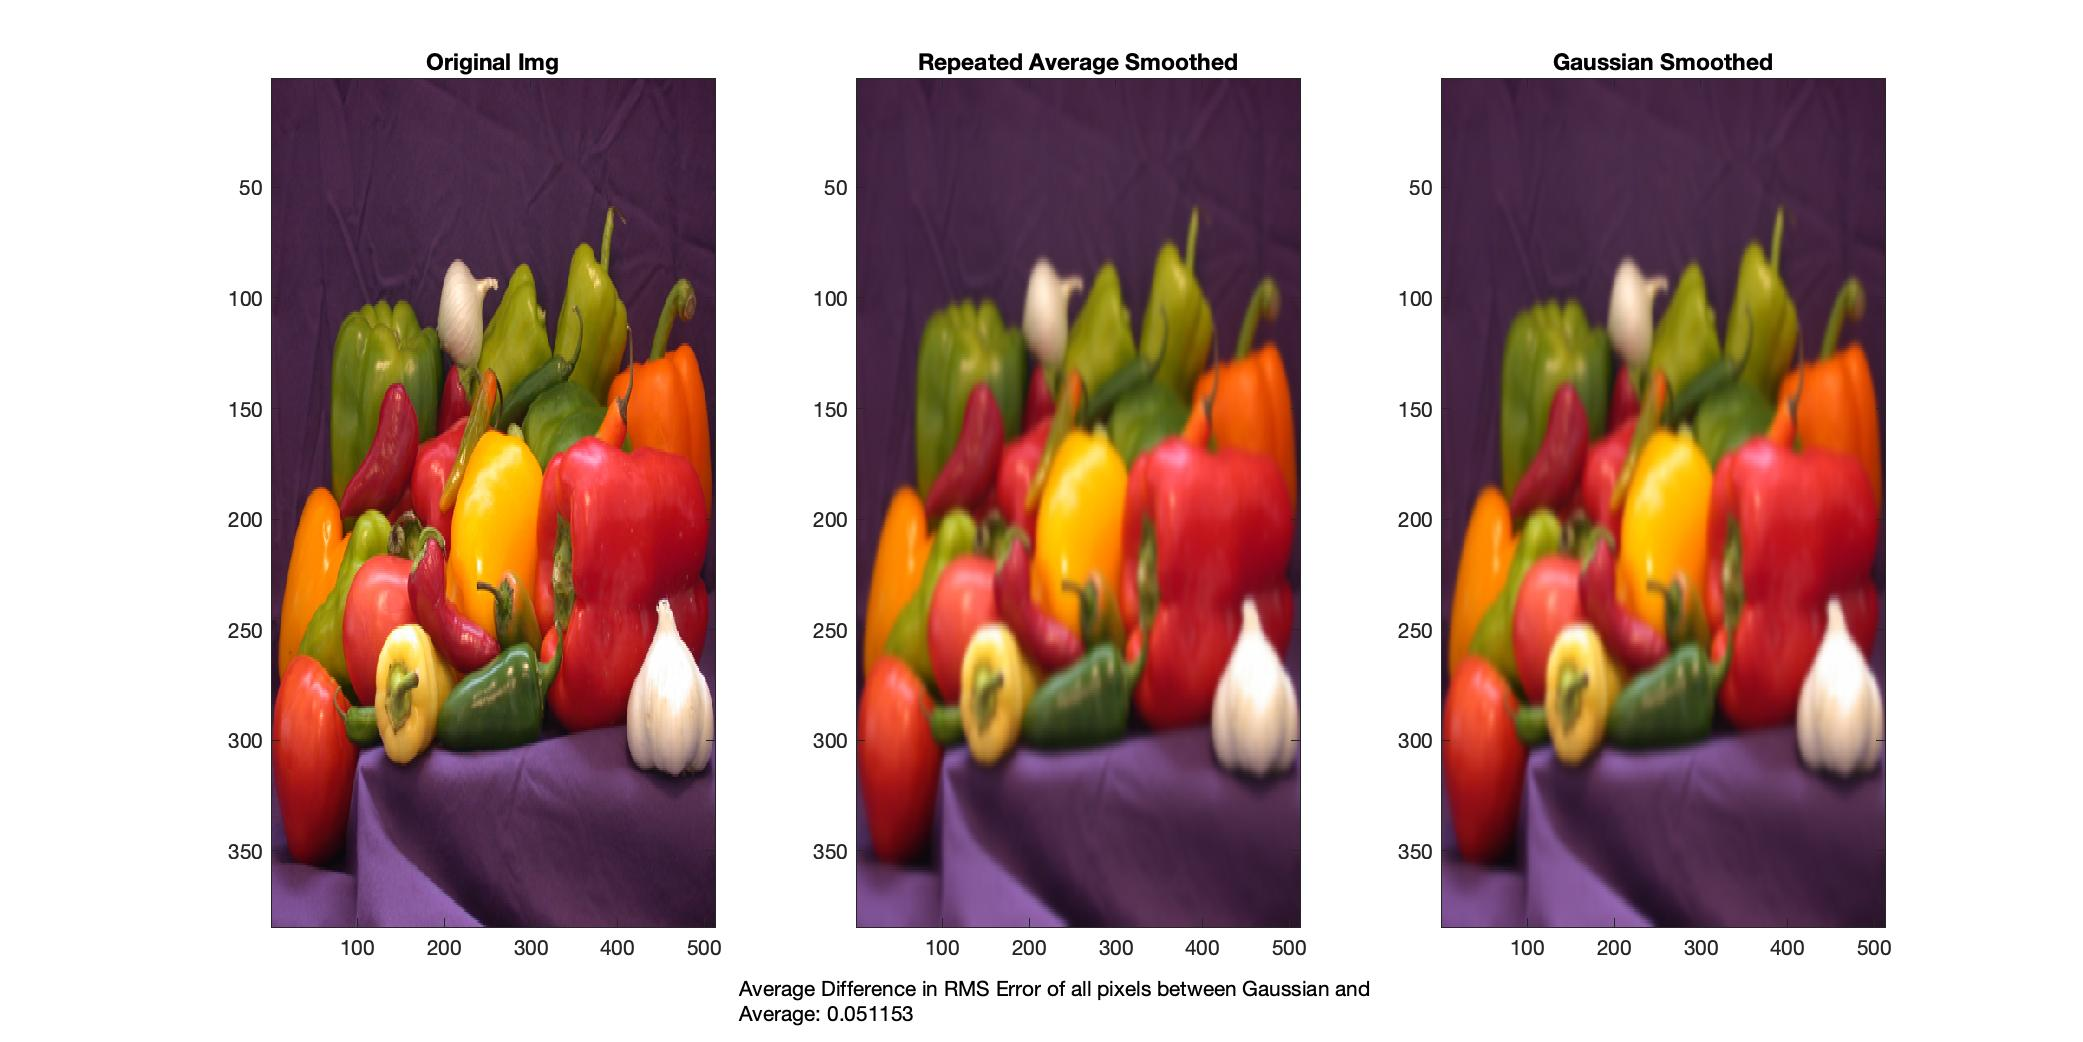
\includegraphics[width=1\textwidth]{Q5_results.jpg}
	\end{figure}
	
	\item
	\begin{enumerate}
		\item The corner detection algorithm had no trouble with all of these transformations. Because all of these were only shifting pixels (either through rotation or translation) or were giving the image more resolution, it had no trouble detecting the same edges as the actual pixel values were not changing. If the image got too small by scaling it down I would imagine eventually it would cause issues for the Harris corner detection algorithm if it ran out of useful pixels to find corners with. Otherwise, these had no noticeable effect on the algorithm.
		
		\begin{figure}[H]
			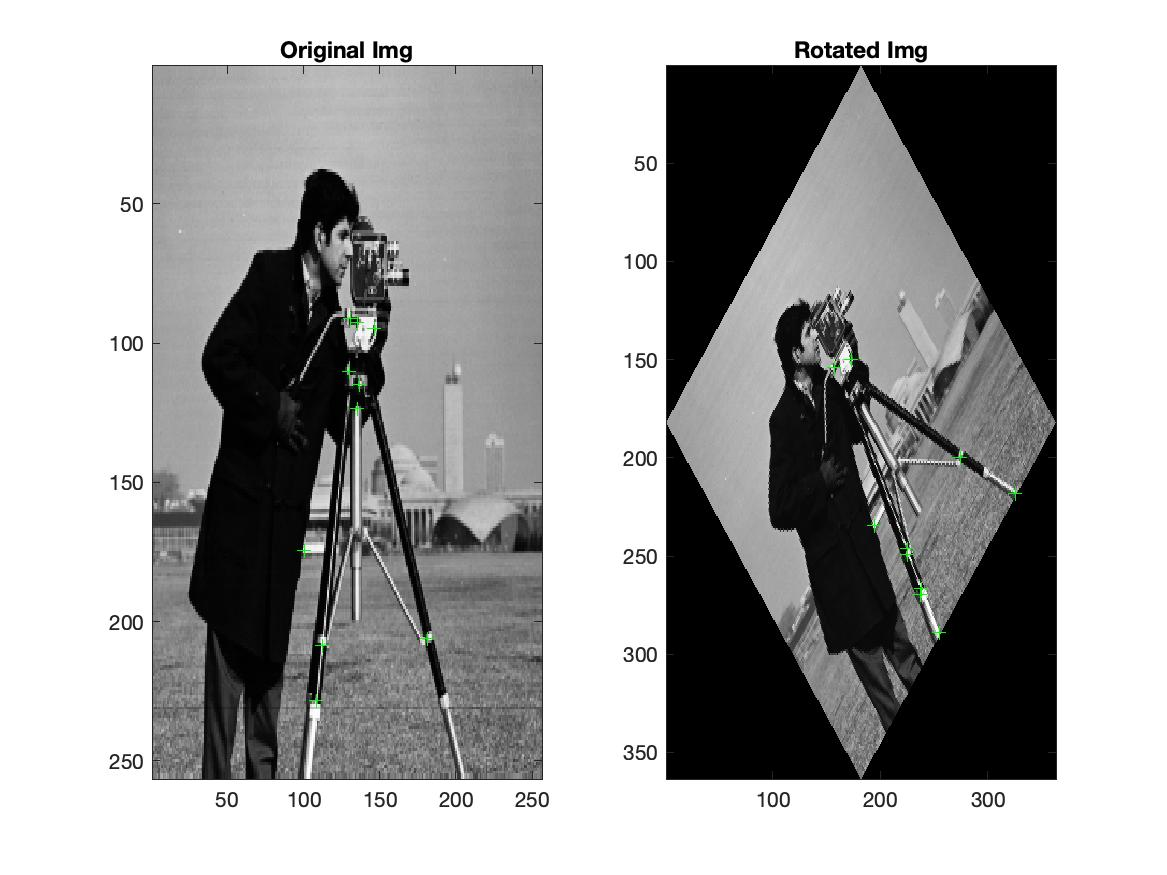
\includegraphics[width=0.5\textwidth]{Q6A_rot_results.jpg}
			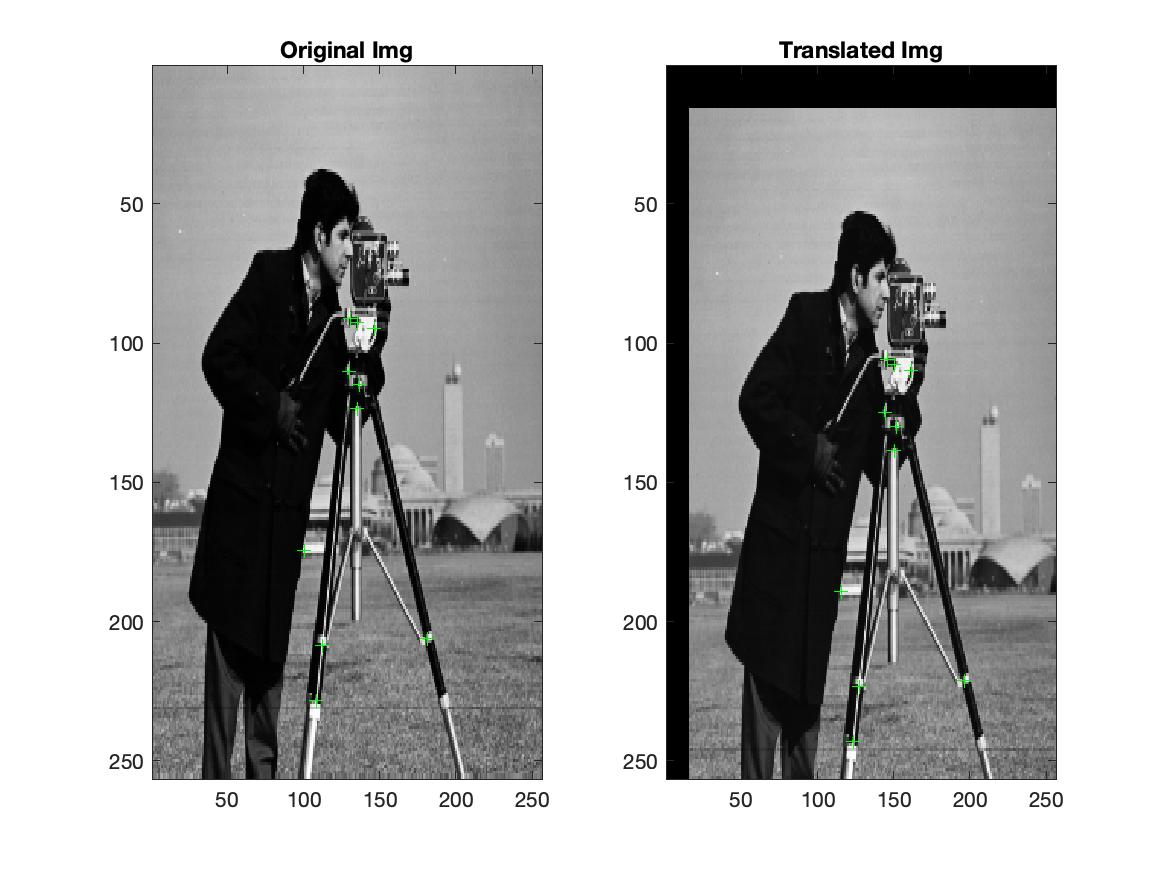
\includegraphics[width=0.5\textwidth]{Q6A_trans_results.jpg}
			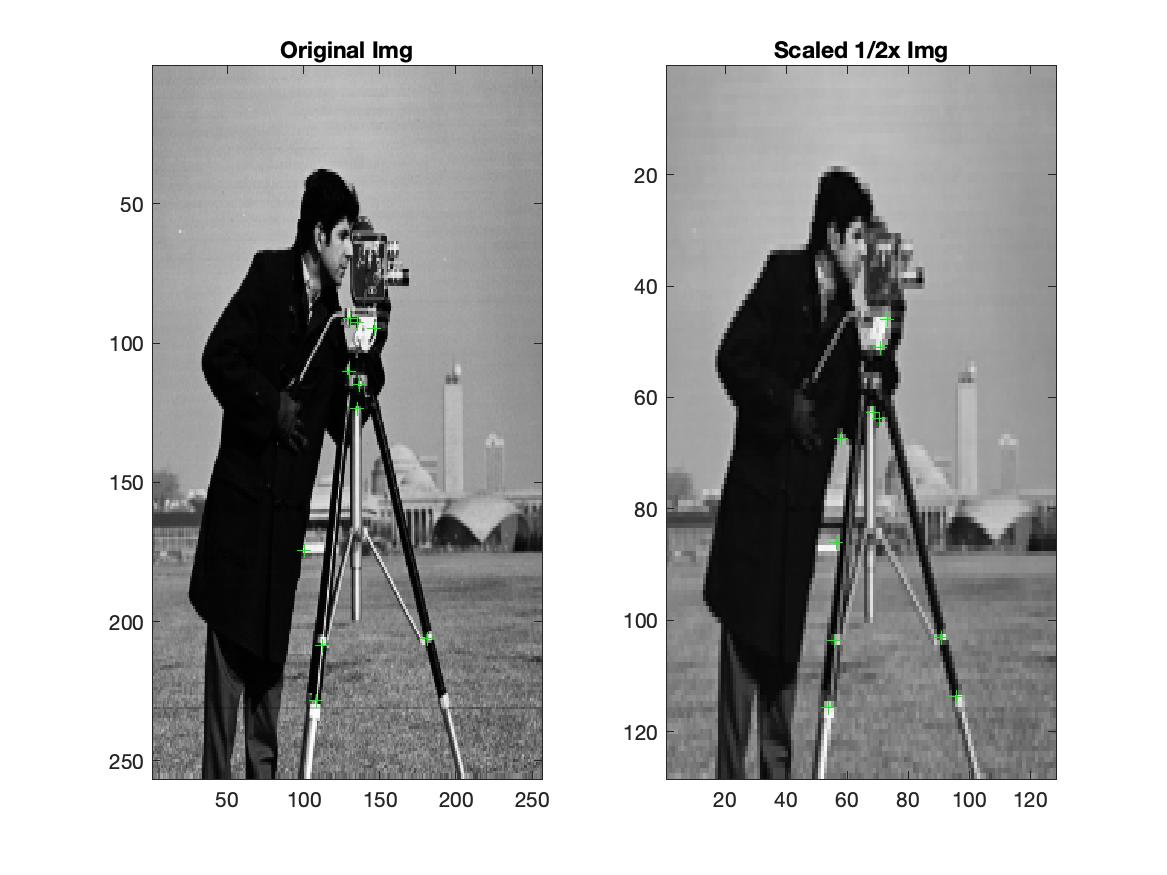
\includegraphics[width=0.5\textwidth]{Q6A_scale_results.jpg}
			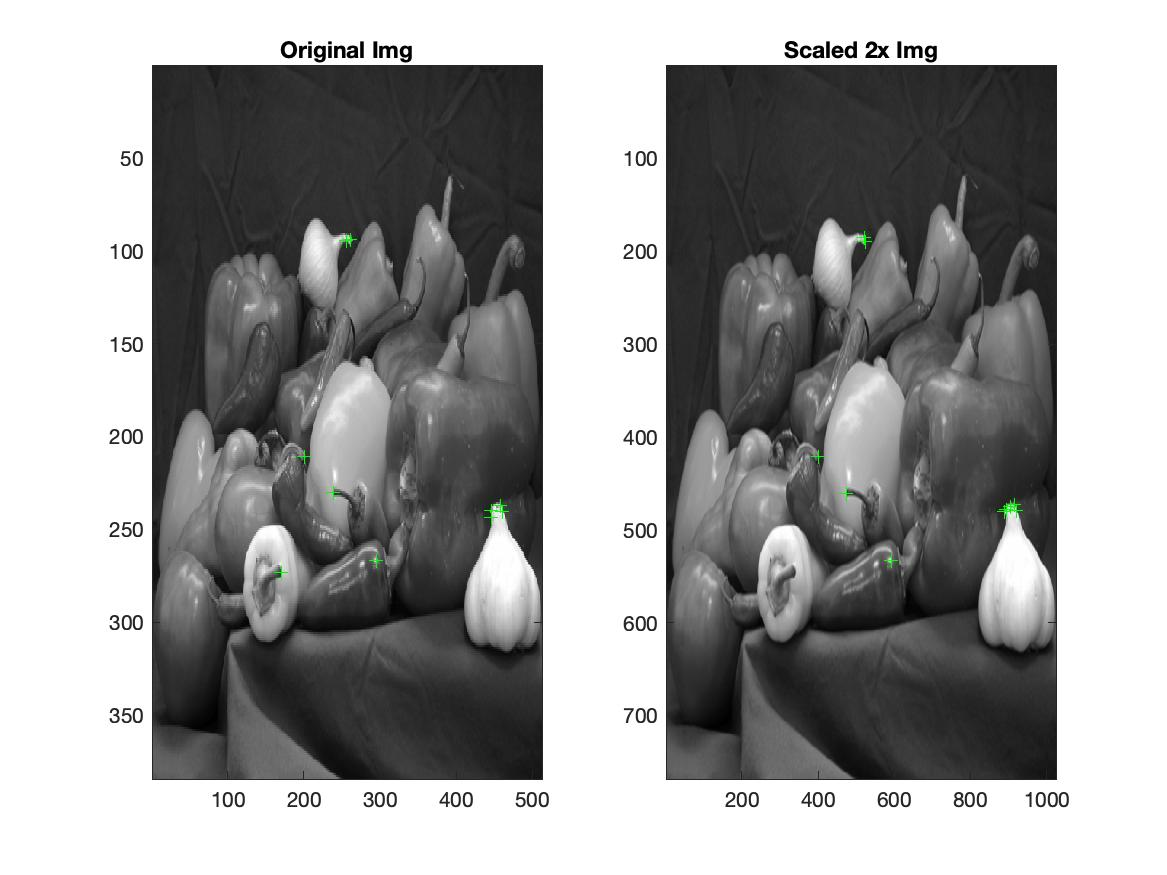
\includegraphics[width=0.5\textwidth]{Q6A_scale2_results.jpg}
		\end{figure}
		
		\item Unlike in part A, these transformations of the images actually changed individual pixel values and therefore had a more noticeable effect on the results of the corner detection algorithm. 
		
		\begin{figure}[H]
			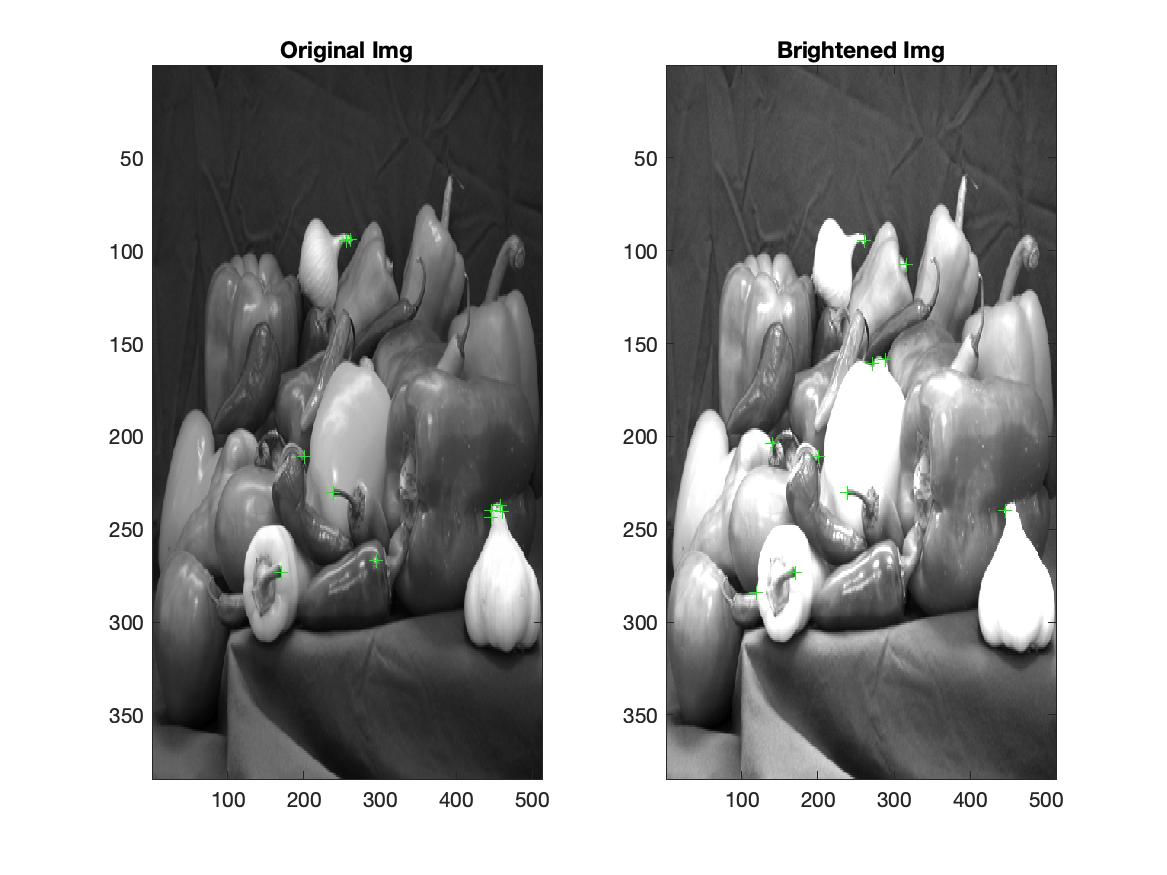
\includegraphics[width=0.5\textwidth]{Q6B_bright_results.jpg}
			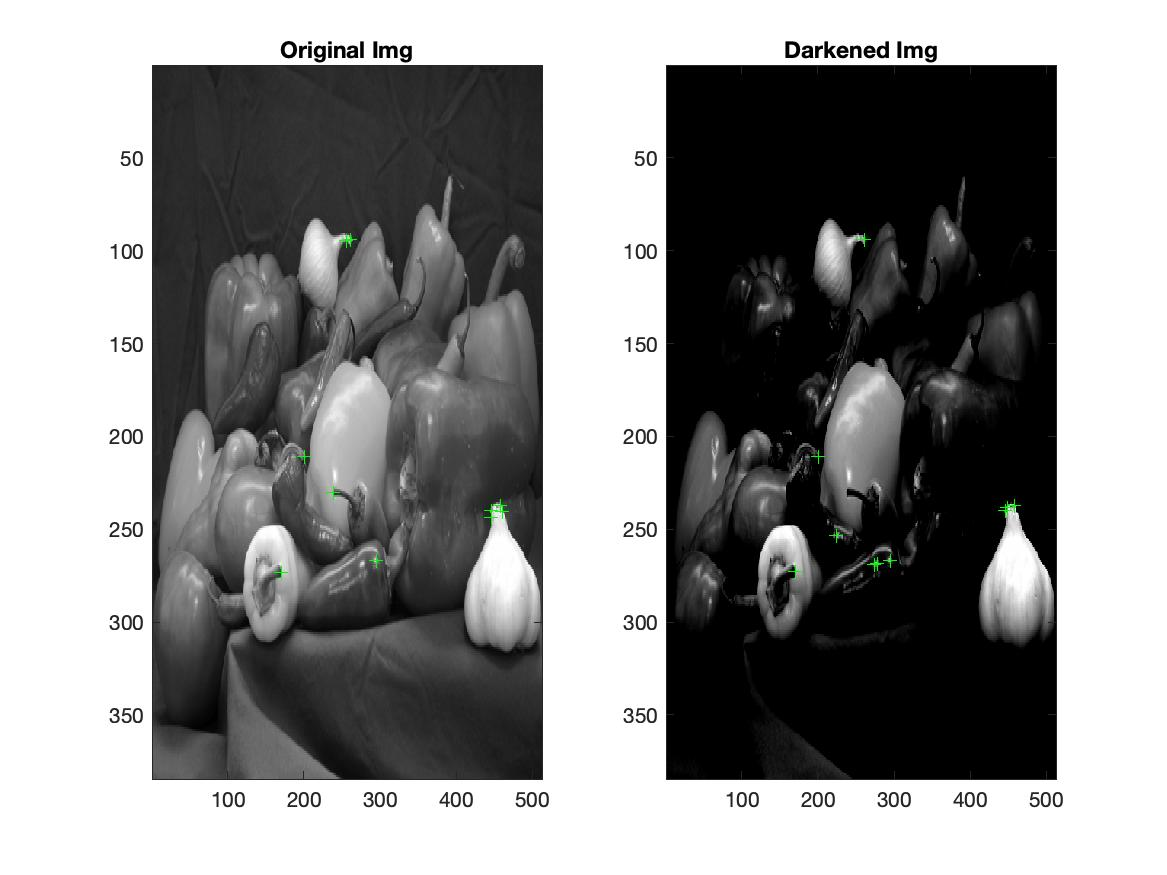
\includegraphics[width=0.5\textwidth]{Q6B_dark_results.jpg}
			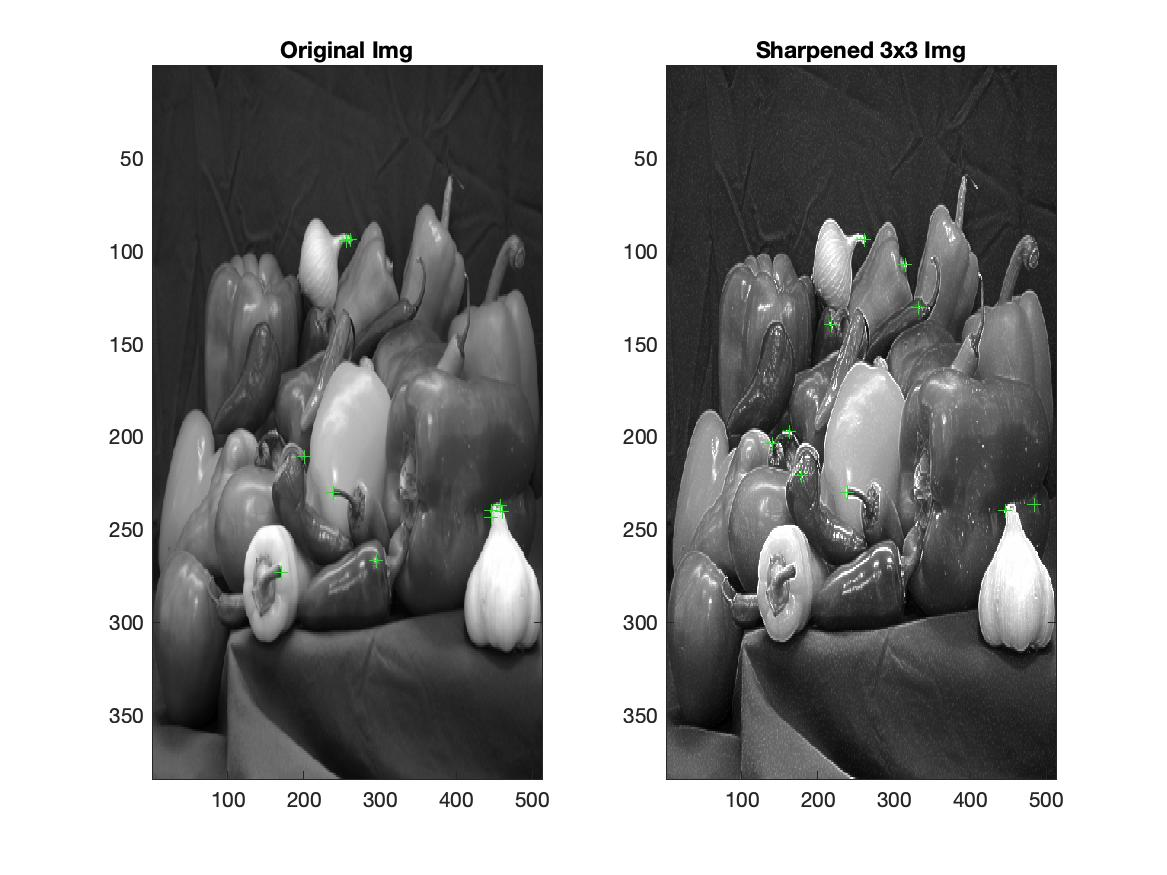
\includegraphics[width=0.5\textwidth]{Q6B_sharp3_results.jpg}
			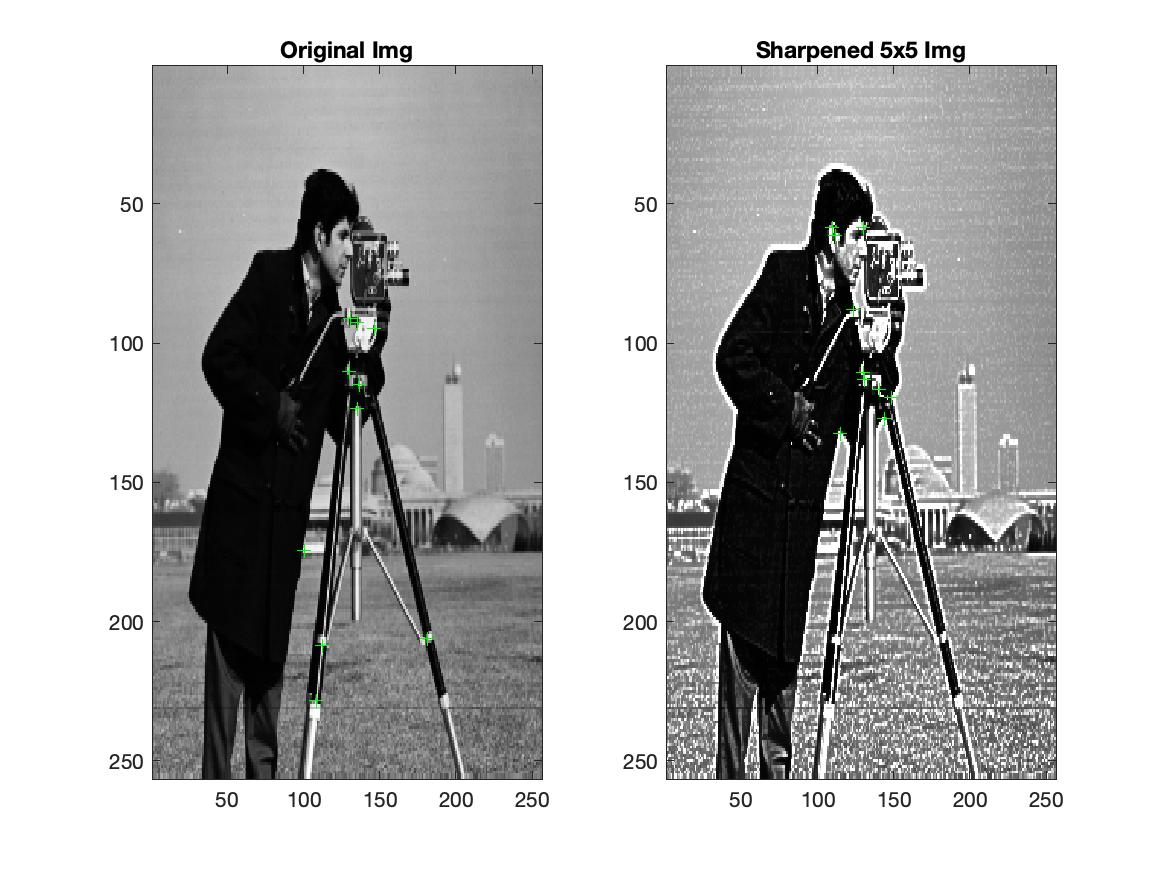
\includegraphics[width=0.5\textwidth]{Q6B_sharp5_results.jpg}
		\end{figure}
		
		
		\item Below is the output of adding increasing amounts of Gaussian noise to a white square on a black background. Gaussian noise 1 (least noise) has a standard deviation of 0.1. Gaussian noise 2 (middle) has a standard deviation of 0.5, and Gaussian noise 3 (most noise) has a standard deviation of 1. In the bar chart, each color bar represents one of the 4 corners we are detecting. As you can see, the lowest level of noise barely effects the corner detection algorithm as all 4 corners are found and have a very low RMS error. For the middle level of noise, the algorithm manages to find 2 corners with low error but the other 2 are way off as seen by the spike in RMS error at standard deviation=0.5 up to above 10. The image with the most noise does not find any of the four corners and all of the corner detection's have very high RMS errors as seen in the bar chart.
		\begin{figure}[H]
			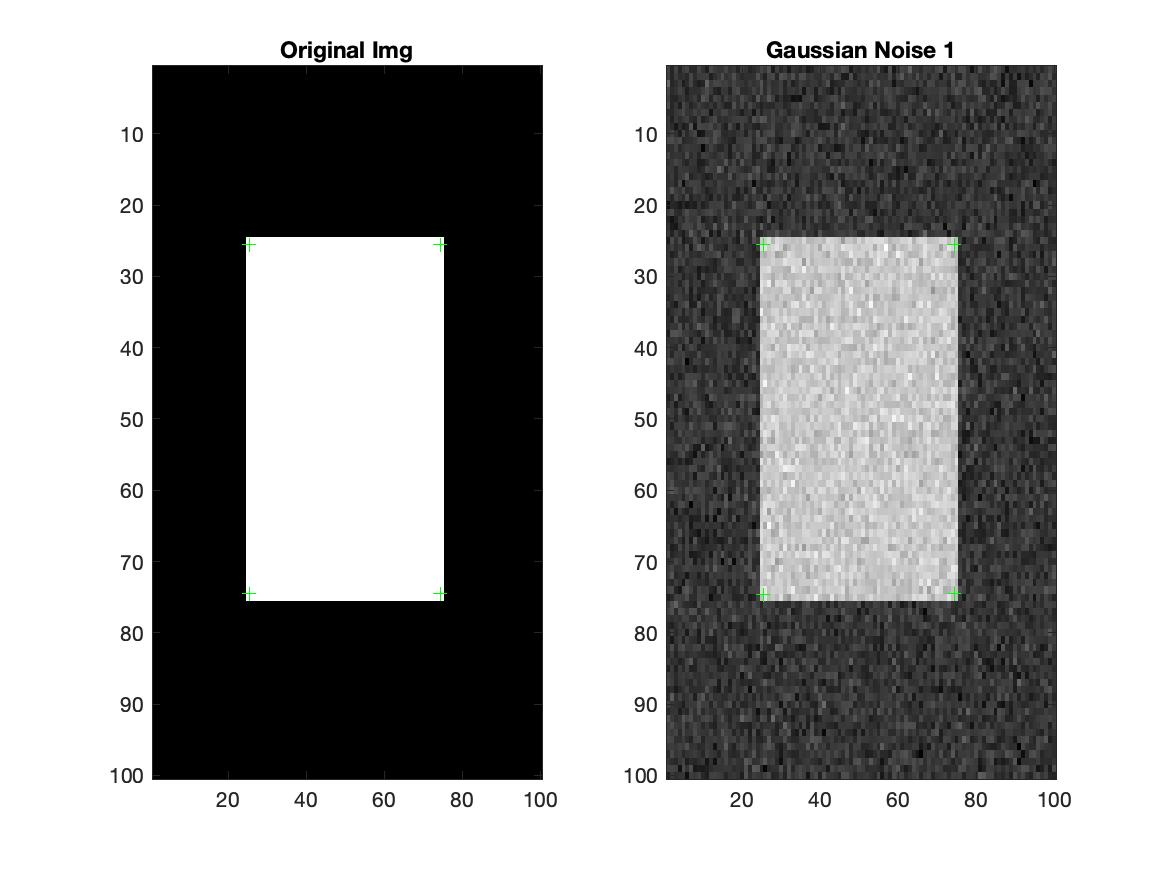
\includegraphics[width=0.5\textwidth]{Q6C_gaussian1_results.jpg}
			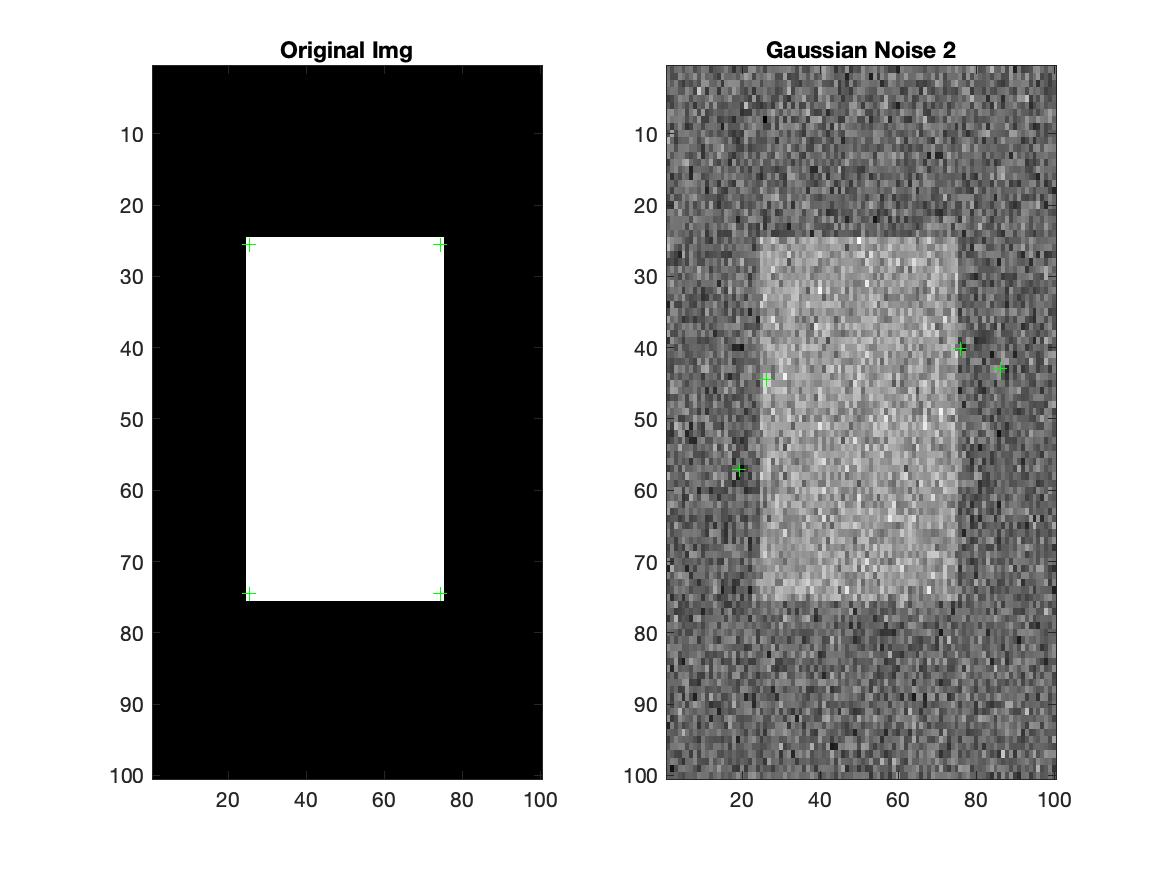
\includegraphics[width=0.5\textwidth]{Q6C_gaussian2_results.jpg}
			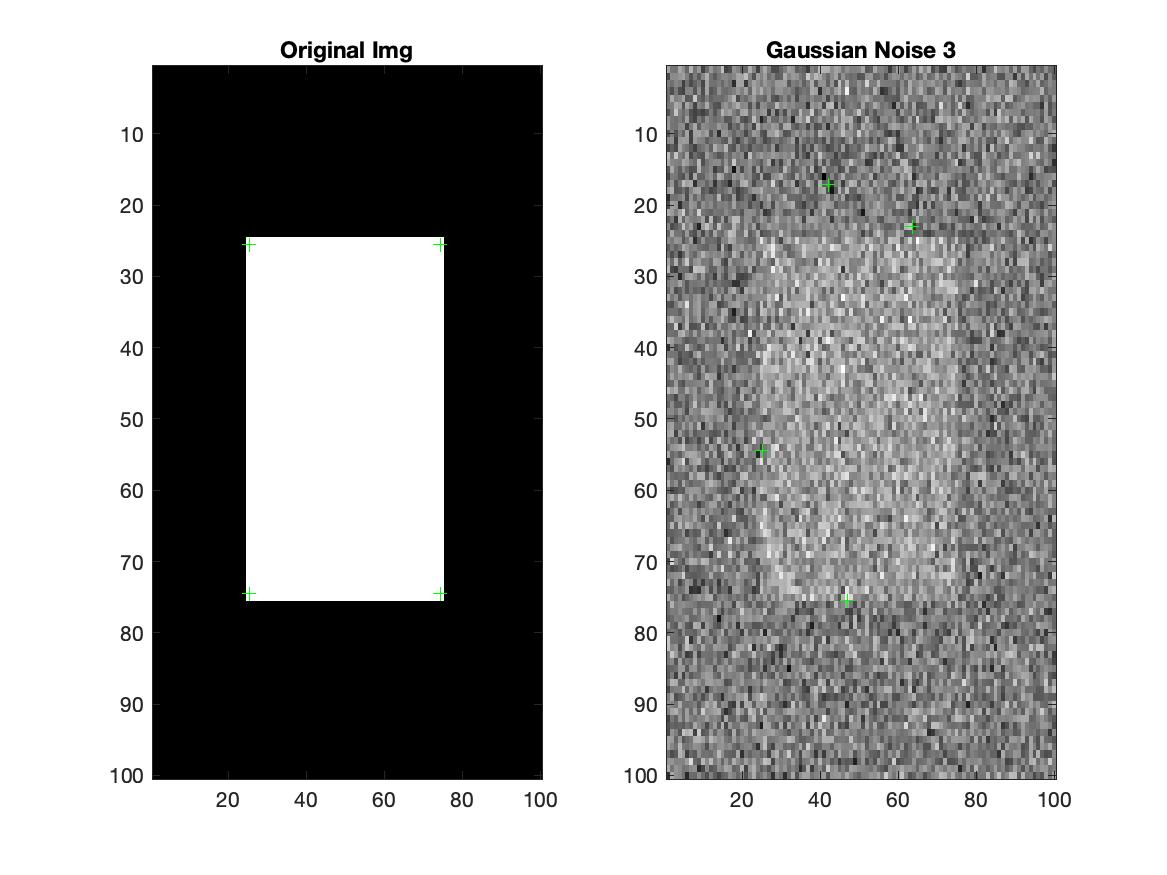
\includegraphics[width=0.5\textwidth]{Q6C_gaussian3_results.jpg}
			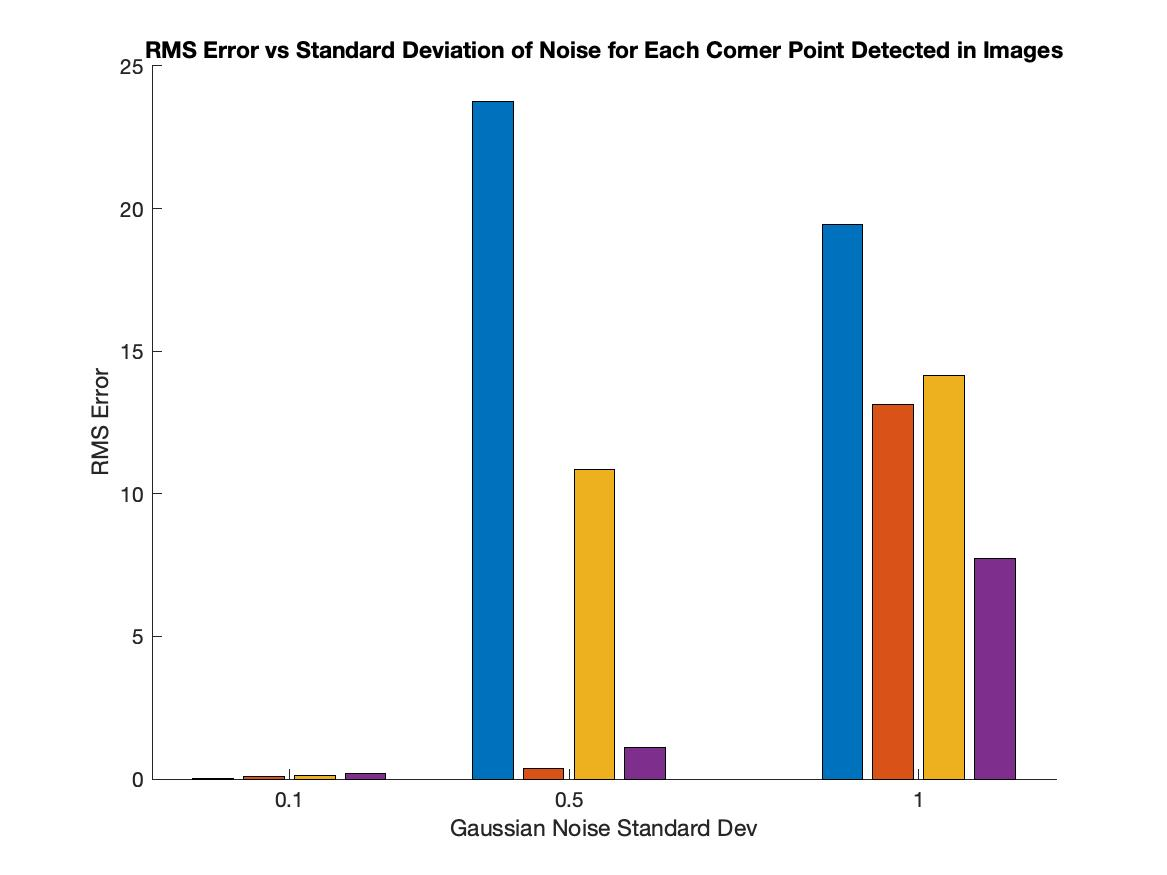
\includegraphics[width=0.5\textwidth]{Q6C_final_distribution_result.jpg}
		\end{figure}
	\end{enumerate}
		
		
\end{enumerate}
%\newpage
%\textbf{Matlab Code}
%\lstinputlisting{hw2.m}
\end{document}

